\documentclass[prd,twocolumn]{revtex4}

\pdfoutput=1

\usepackage{graphicx}
\usepackage{dcolumn}
\usepackage{bm}
\usepackage{amssymb,amsmath,bm}  
\usepackage{color}
\usepackage{hyperref}
\usepackage{multirow}
\usepackage[utf8]{inputenc}
\usepackage{balance}
\usepackage{enumitem}
\usepackage{lipsum}
\newcommand{\uKam}{\mu\text{K-arcmin}}
\newcommand{\nv}{\hat{\bf n}}
\newcommand{\jcap}{JCAP}
\newcommand{\mnras}{MNRAS}
\newcommand{\aap}{A\&A}
\newcommand{\aaps}{A\&AS}
\newcommand{\apjs}{ApJS}
\newcommand{\apjl}{ApJL}
\newcommand{\aj}{Astron. Journal}
\newcommand{\pasp}{Publications of the ASP}
\newcommand{\nar}{New Astronomy Review}
\newcommand{\procspie}{Proceedings of the SPIE}
\newcommand{\TODO}[1]{{\bf TODO:} \textcolor{red}{#1}}
\newcommand{\zph}{z_{\rm ph}}
\newcommand{\fsh}{\hat{\sf F}}
\newcommand{\cov}{\hat{\sf C}}

\begin{document}
\title{Calibrating photometric redshifts with intensity mapping observations}
\author{All of us$^1$}
\affiliation{$^{1}$University of Wherever}

\begin{abstract}
  \TODO{\lipsum[1]}
\end{abstract}

  \date{\today}
  \maketitle

\section{Introduction}\label{sec:intro}
  \TODO{\lipsum[2]}
% This method was originally proposed as a way to calibrate photometric
%    redshift distributions through cross-correlations with an overlapping spectroscopic survey
%    with no requirement on completeness or sampling of colour space.
  
    \begin{figure*}
      \centering
      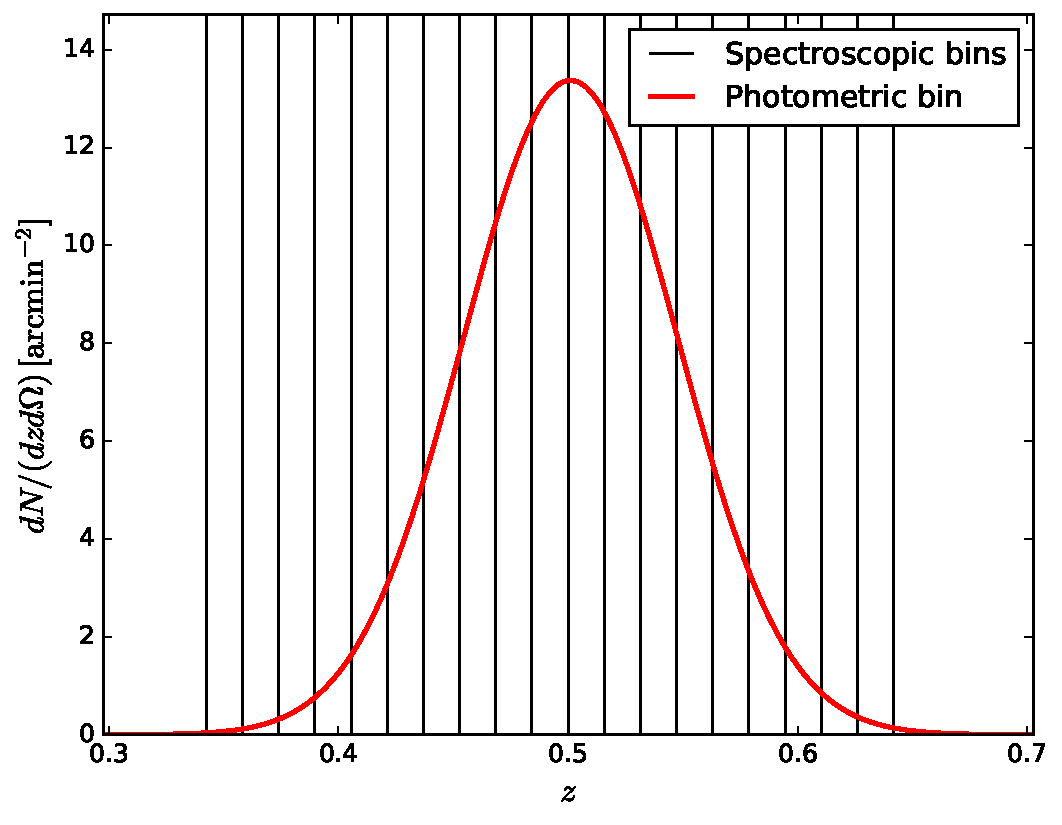
\includegraphics[width=0.49\textwidth]{bins}
      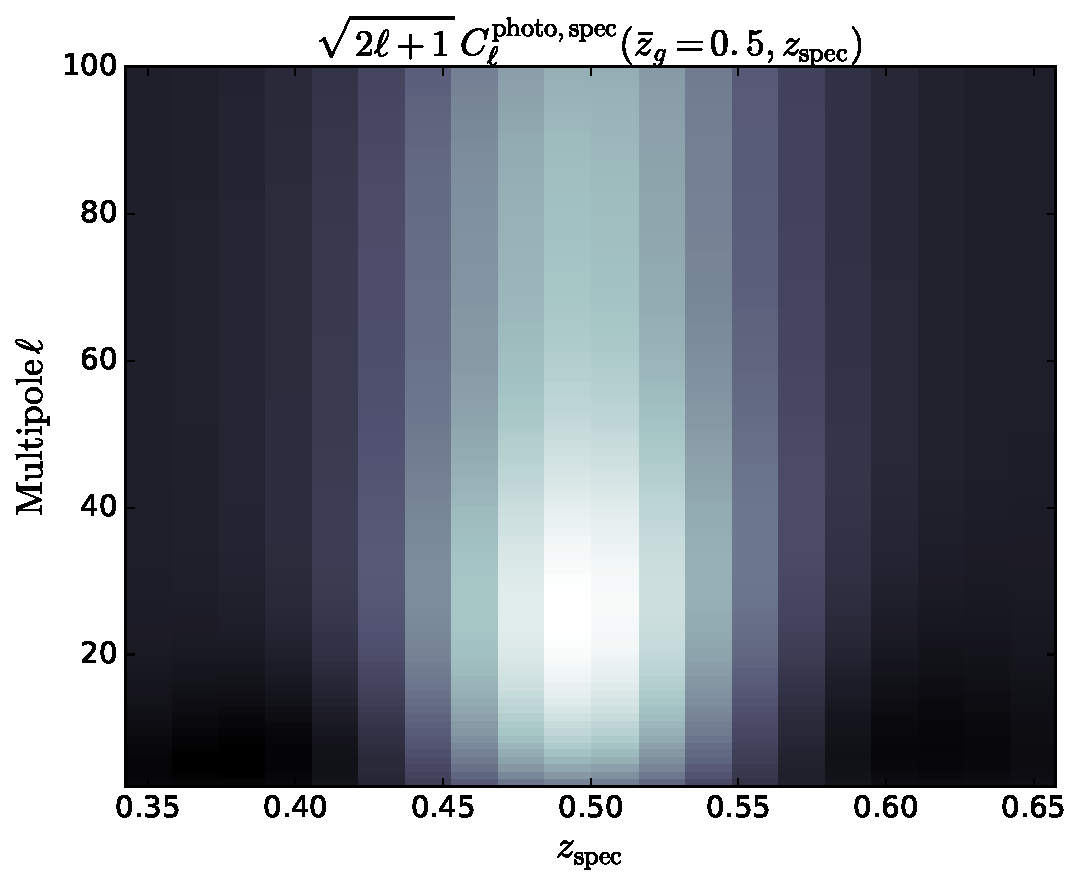
\includegraphics[width=0.49\textwidth]{xcorr_map}
      \caption{{\sl Left panel:} example of a redshift bin for a photometric survey and the redshift
               bins chosen for an overlapping spectroscopic survey.
               {\sl Right panel:} amplitude of the cross-correlation with an overlapping spectroscopic
               survey as a function of spectroscopic redshift bin ($x$ axis) and angular scale
               ($y$ axis). The amplitude of the cross-correlation traces the redshift distribution,
               and can therefore be used to constrain it.}
      \label{fig:clustred_example}
    \end{figure*}
\section{Formalism}\label{sec:method}
  \subsection{Clustering-based photo-$z$ calibration}\label{ssec:method.clustred}
    Consider two galaxy samples with redshift distributions $\phi_i(z)$ ($i=\{1,2\}$),
    and let $a^i_{\ell m}$ be the harmonic coefficients of their projected overdensity
    of counts on the sky. Their cross-correlation is given by:
    \begin{align}
      &\langle a^i_{\ell m}(a^j_{\ell m})^*\rangle=N^{ij}_\ell+S^{ij}_\ell\\\label{eq:cl1}
      &S^{ij}_\ell=\frac{2}{\pi}\int dz \int dz'\,\phi_i(z)\phi_j(z')\times\\\nonumber
      &\times\int dk\,k^2\,b_i(z)b_j(z')P_m(k,z,z')\,j_\ell(k\chi(z))\,j_\ell(k\chi(z')),
    \end{align}
    where $P_m$ is the matter power spectrum, $j_\ell(x)$ is a spherical Bessel function,
    $N^{ij}_\ell$ is the cross-noise power spectrum between samples $i$ and $j$, $b_i$
    is the linear bias of the $i$-th sample and we have neglected redshift-space distortions
    and all other sub-dominant contributions to the observed power spectrum. In the Limber
    approximation ($j_\ell(x)\rightarrow\sqrt{\pi/(2\ell+1)}\delta^\mathcal{D}(\ell+1/2-x)$),
    this simplifies to:
    \begin{equation}\label{eq:cl2}
      S^{ij}_\ell=\int dk\,P_m(k,z_\ell)\,\frac{H^2(z_\ell)b^i(z_\ell)b^j(z_\ell)}{\ell+1/2}
      \phi_i(z_\ell)\phi_j(z_\ell),
    \end{equation}
    where $\chi(z_\ell)\equiv(\ell+1/2)/k$.

    For the purposes of this discussion, the most important feature of Equation \ref{eq:cl2}
    is the fact that the amplitude of the cross-correlation is proportional to the overlap
    between the redshift distributions of those samples. This is especially relevant if one
    of the samples has good radial resolution, in which case it can be split into narrow bins
    of redshift. The cross-correlations of all narrow bins with the other sample will
    therefore trace the amplitude of its redshift distribution, and can effectively be used
    to constrain it. This is illustrated in Fig. \ref{fig:clustred_example}, which shows the
    cross-power spectrum between a Gaussian photo-$z$ bin of width $\sigma=0.05$ and a set
    of narrow redshift bins ($\delta z\sim0.002$).

    Different recipes have been formulated to carry out this kind of analysis, such as the
    optimal quadratic estimator method of \cite{2013MNRAS.433.2857M}. The forecasts
    presented here will interpret the redshift distribution (in a parametric or
    non-parametric form) as a set of extra nuisance parameters, on which we will carry out
    the Fisher matrix analysis described in Section \ref{ssec:method.fisher}. Thus, even
    though our results will be optimistic in as much as the Fisher matrix saturates the
    Rao-Cramer bound, they will account for all correlations between redshift distribution
    parameters and with the cosmological parameters, as well as the presence of
    redshift-space distortions and magnification bias (effects that have been overseen in
    previous works).

    For the purposes of estimating the ability of future surveys to calibrate photometric
    redshift distributions through cross-correlations, we will always consider an individual
    redshift bin for a photometric sample with unknown distribution together with a set of
    overlapping narrow redshift bins of spectroscopic galaxies or intensity mapping
    observations. Let $N^p(z)$ be the overall true redshift distribution of the photometric
    sample, and let $p(\zph|z)$ be the conditional distribution for a photo-$z$ $\zph$
    given the true redshift $z$. Then, the redshift distribution in a photo-$z$ redshift bin
    $b$ with bounds $z_b^i<\zph<z_b^f$ is given by
    \begin{equation}\label{eq:phz_dist}
      \phi_b(z)\propto N^p(z)
      \int_{z_b^i}^{z_b^f}d\zph\,p(\zph|z).
    \end{equation}
    In what follows we will consider 3 degrees of complexity in terms of describing the
    unknown redshift distribution:
    \begin{enumerate}
      \item We will assume Gaussianly-distributed photo-$z$s with a given variance ($\sigma_z^2$)
        and bias $\Delta z$:
        \begin{align}\nonumber
          p(\zph|z)&\equiv \mathcal{N}(\zph-\Delta z;z,\sigma_z)\\\label{eq:photoz_gaussian}
          &\equiv\frac{\exp\left[-\frac{1}{2}\frac{(\zph-z-\Delta z)^2}{\sigma_z^2}\right]}{\sqrt{2\pi\sigma_z}},
        \end{align}
        and we will assume that the uncertainty in the redshift distribution is fully
        described by $\Delta z$ and $\sigma_z$.
      \item We will introduce hard tails in the photo-$z$ distribution (possibly caused
        by catastrophic outliers) and parametrize it by a Voigt profile, combining a
        Gaussian and Cauchy distributions. The tails are thus parametrized by $\gamma_L$,
        the half-width at half-maximum of the Cauchy component. The exact form of the
        Voigt profile used here is described in Appendix \ref{app:voigt}.
      \item We will use a non-parametric form for $\phi_b(z)$, given as a piecewise function with
        a free amplitude for each spectroscopic redshift bin.
    \end{enumerate}
    Our assumed fiducial value for $\Delta z$, $\sigma_z$ and $\gamma$, as well as the binning scheme
    used are described in Section \ref{ssec:method.phz}.

    We finish this section by noting that the use of cross-correlations with spectroscopic surveys or
    intensity mapping observations for photo-$z$ calibration is not limited to the measurement of
    the redshift distribution of a given galaxy sample, but that they can also be used to improve the
    precision of photometric redshift estimates for individual galaxies (e.g. \cite{2012MNRAS.425.1042J}). 
    Although we leave the discussion of this possibility for future work, we describe a Bayesian
    formalism for this task in Appendix \ref{app:ind_phz}.
    
  \subsection{Photometric redshift surveys}\label{ssec:method.phz}
    \begin{figure}
      \centering
      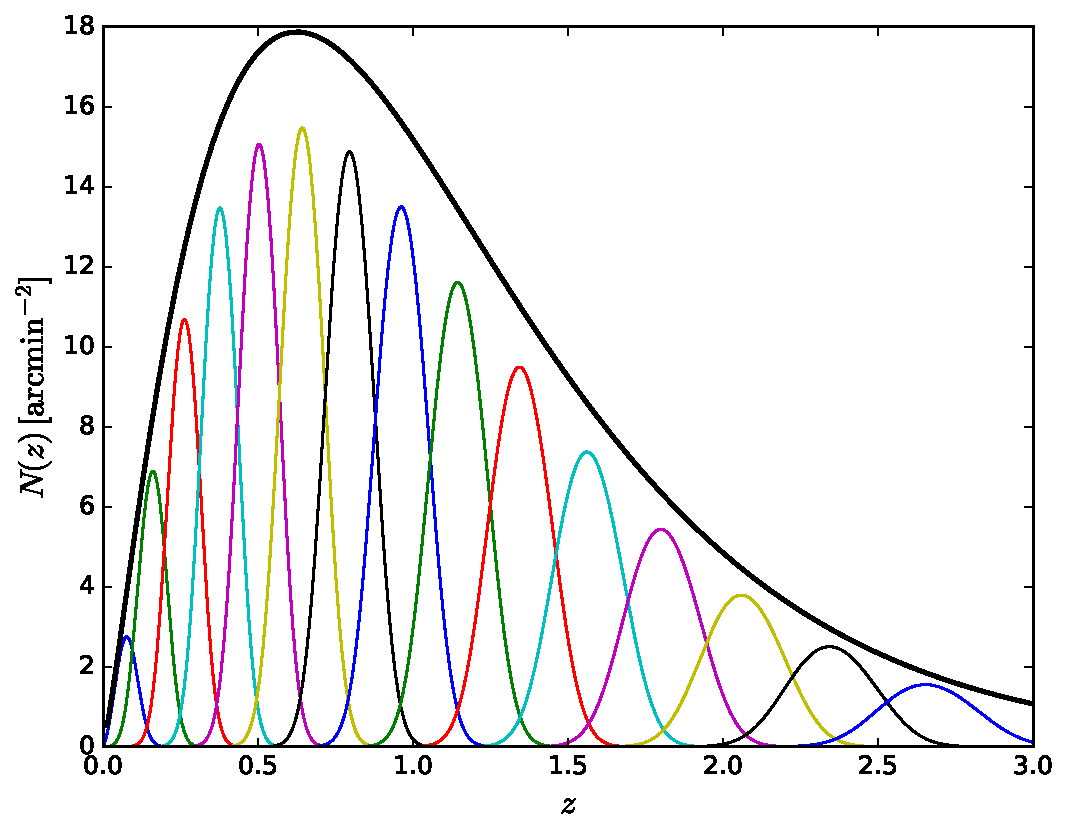
\includegraphics[width=0.49\textwidth]{nz_lsst}
      \caption{Angular number density of galaxies as a function of redshift for the LSST
                gold sample (solid black line). The colored lines in show the window functions
                of the 15 redshift bins considered here.}
      \label{fig:nz_lsst}
    \end{figure}
    This section describes the model used here for a LSST-like photometric redshift survey.
    As in \cite{2015PhRvD..92f3525A}, we base our description of the number density of sources
    and their magnification bias on the measurements of the luminosity function of
    \cite{2006A&A...448..101G}, with $k$-corrections computed with {\tt kcorrect}
    \cite{2007AJ....133..734B}. We assume a magnitude cut of $25.3$ in the $i$ band, corresponding
    to the so-called ``gold'' sample \cite{2009arXiv0912.0201L}. Unlike \cite{2015PhRvD..92f3525A},
    and for simplicity, we will consider a single galaxy population,
    instead of splitting it into ``red'' and ``blue'' sources. The resulting redshift
    distribution is shown by the solid black line in Figure \ref{fig:nz_lsst}.

    We model the linear galaxy bias as a function of redshift as $b(z)=1+0.84z$, based
    on the simulations of \cite{2004ApJ...601....1W}, and quoted in the LSST science book
    \cite{2009arXiv0912.0201L}.
    
    The photometric redshift requirement for the gold sample as stated in the LSST science
    book are $\sigma_z/(1+z)<0.05$, with a goal of $0.02$. Here we have taken a conservative
    estimate, assuming a standard deviation $\sigma_z=0.03(1+z)$. We then split the full
    sample into redshift bins with a width given by $3\times\hat{\sigma}_z$, where
    $\hat{\sigma}_z$ is the photo-$z$ variance at the bin centre. This binning scheme is
    chosen to reduce the correlation between bins induced by the tails of the photo-$z$
    distribution, and results in the 15 redshift bins shown in Fig. \ref{fig:nz_lsst} (where
    the redshift distributions are computed with Eq. \ref{eq:phz_dist}. Our fiducial
    photo-$z$ model will assume unbiased Gaussian distributions, fully determined by
    $\sigma_z$. When considering biased and hard-tailed distributions parametrized as
    Voigt profiles we will assume $\Delta z=0$ and $\gamma_L=0$ for our fiducial
    model.

  \subsection{Intensity mapping}\label{ssec:method.imap}
    \begin{table}
      \centering{
      \renewcommand*{\arraystretch}{1.2}
      \begin{tabular}{|c|c|c|}
        \hline
        Experiment     & SKA / MeeKAT     & HIRAX              \\
        \hline
        $T_{\rm inst}$ & 25K            & 50 K               \\
        $t_{\rm tot}$  & 10000 / 4000 h & $2.8\times10^4$ h  \\
        $N_{\rm dish}$ & 197 / 64       & 1024 ($32\times32$)\\
        $D_{\rm dish}$ & 15 / 13.5 m    & 6 m                \\
        freq. range    & 350-1050 MHz   & 400-800 MHz    \\
        $f_{\rm sky}$  & 0.4 / 0.1      & 0.4   \\
        \hline
      \end{tabular}}
      \caption{Experimental specifications assumed for SKA, MeerKAT and HIRAX. The baseline
               distributions for each experiment are described in Sections
               \ref{sssec:method.imap.ska} and \ref{sssec:method.imap.hirax}.}
      \label{tab:im_exp}
    \end{table}
    Intensity mapping (IM) is a novel observational technique that tries to circumvent the
    long integration times needed to obtain reliable spectroscopic redshifts for individual
    objects through an approach that is transverse to that used by photometric surveys.
    The idea \TODO{cites} is to observe the unresolved combined emission of many line-emitting
    sources in a relatively wide pixel at different frequencies. The signal-to-noise ratio
    of the corresponding line emission is much stronger than that of the individual sources,
    and thus, combining the intensity measured across the sky and relating the intensity
    observed at a given frequency to the rest-frame wavelength of the emission line it is
    possible to produce three-dimensional maps of the density of the line-emitting species.
    This technique is particularly appealing for isolated spectral lines, as is the case
    of the 21cm line caused by the spin-flip transition in neutral Hydrogen atoms (HI),
    and thus HI intensity mapping has been proposed as an ideal method to cover vast
    volumes at relatively low cost.
    
    A number of experiments have been proposed to carry out IM measurements of the baryon
    acoustic oscillation scale, such as \TODO{add experiments with references}. The 
    different instrumental approaches to IM can be broadly classified into two camps:
    \begin{itemize}
      \item {\sl Interferometers:} the sky emission is measured by a set of antennas, and
      the measurements of pairs of antennas separated by a given baseline ${\bf d}$ are
      cross-correlated to produce the measurement of an angular Fourier mode with scale
      ${\bf l}\sim2\pi{\bf d}/\lambda$ (where $\lambda$ is the observed wavelength).
      The intensity map is then reconstructed by combining pairs with different baselines.
      \item {\sl Single-dish:} in this case the sky emission is measured and auto-correlated
      by individual antennas. A band-limited intensity map with a resolution
      $\delta\theta\sim\lambda/D_{\rm dish}$ is then produced by varying the antenna pointing,
      where $D_{\rm dish}$ is the antenna diameter.
    \end{itemize}
    The expressions for the noise power spectrum for both cases are derived in Appendix
    \ref{app:noise_im}, and can be summarized as:
    \begin{equation}\label{eq:nl_im}
      N^\nu_{\bf l}=\frac{T_{\rm sys}^24\pi f_{\rm sky}}{\eta^2\Delta\nu t_{\rm tot}}
      \left\{\begin{array}{ll}
              \frac{1}{N_{\rm dish}B^2({\bf l})}, & \text{single dish}\\
              \frac{\Omega_p}{N_d({\bf d}={\bf l}\lambda/(2\pi))\lambda^2}, & \text{interferometer}.
             \end{array}\right.
    \end{equation}
    Here $T_{\rm sys}$ is the system temperature, given as a combination of instrumental and sky
    temperature (see Appendix \ref{app:noise_im}), $f_{\rm sky}$ is the sky fraction covered
    by the observations, $\eta^2$ is the antenna efficiency\footnote{$\eta$ is defined as the
    ratio of the effective to real antenna area.}, $\Delta\nu$ is the band width in that channel,
    $t_{\rm tot}$ is the total observation time for the survey, $N_{\rm dish}$ is the number of
    dishes, $B({\bf l})$ is the harmonic transform of the antenna beam, $N_d({\bf d})$ is the
    distribution of baselines and $\Omega_p$ is the solid angle covered per pointing. For all
    experiments discussed here we will assume $\eta=1$, Gaussian beams so that
    $B({\bf l})=\exp[-l(l+1)\theta_{\rm FWHM}^2/(16\log2)]$, and $\Omega_p=\theta_{\rm FWHM}^2$,
    where $\theta_{\rm FWHM}$ is the beam full-width at half maximum, which will approximate
    as $\theta_{\rm FWHM}=1.22\lambda/D_{\rm dish}$. Note that the baseline distribution $N_d$
    is normalized such that:
    \begin{equation}
      \frac{N_{\rm dish}(N_{\rm dish}-1)}{2}=\int d{\bf d}^2\,N_d({\bf d}),
    \end{equation}
    where $N_{\rm dish}(N_{\rm dish}-1)/2$ is the total number of independent baselines.
    
    Given their expected full overlap with LSST, we will consider here the two main currently
    envisaged southern-hemisphere intensity mapping experiments: SKA (and its pathfinder,
    MeerKAT) and HIRAX.


    \TODO{Introduce and describe SKA and HIRAX. See specifications in Table \ref{tab:im_exp}.}
    
    \subsubsection{SKA and MeerKAT}\label{sssec:method.imap.ska}
      \TODO{Matt?}
      
    \subsubsection{HIRAX}\label{sssec:method.imap.hirax}
      \TODO{Kavi?}
      
    \subsubsection{Generic IM experiment}\label{sssec:method.imap.generic}
    
    Besides SKA and HIRAX we will also explore the capabilities of generic single-dish and
    interferometer experiments in terms of photo-$z$ calibration. We will parametrize these
    in terms of their instrument temperature $T_{\rm inst}$ and the minimum or maximum angular
    scale that they are able to probe. On the one hand, single-dish experiments are limited
    on small angular scales by the beam size, which is governed by the dish diameter
    $D_{\rm dish}$. On the other hand, interferometers are limited on large scales by their
    shortest baseline $d_{\rm min}$ which, assuming a closed-pack configuration, is also
    given by $d_{\rm min}=D_{\rm dish}$. Thus we will explore the capabilities of generic
    experiments in the $T_{\rm inst}-D_{\rm dish}$ plane, and in the case of interferometers
    we will assume a flat baseline distribution \TODO{cite}:
    \begin{equation}
      N_d(d)=\left\{\begin{array}{cc}
                      \frac{N_{\rm dish}(N_{\rm dish}-1)}{2\pi(d_{\rm max}^2-D^2_{\rm dish})}
                      & {\rm if}\,D_{\rm dish}<d\leq d_{\rm max},\\
                      0 & \text{otherwise}
                    \end{array}\right.
    \end{equation}

    
    \TODO{Discuss foregrounds.}
 
  \subsection{Spectroscopic surveys}\label{ssec:method.spec}
    \begin{figure}
      \centering
      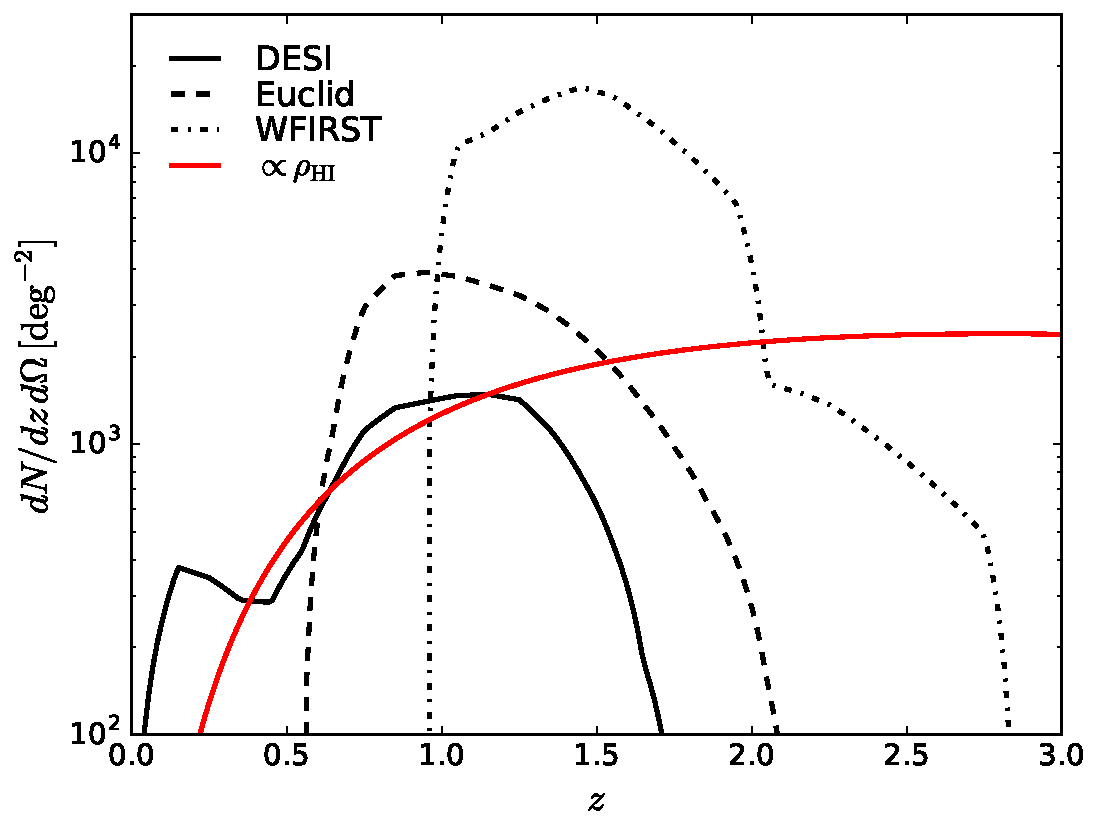
\includegraphics[width=0.49\textwidth]{nz_spec}
      \caption{Angular number density of galaxies as a function of redshift for the three
               spectroscopic surveys considered here: DESI (solid), Euclid (dashed) and
               WFIRST (dot-dashed).}
      \label{fig:nz_spec}
    \end{figure}
    In order to showcase the possibility of calibrating redshift distributions through
    cross-correlation with future intensity mapping experiments we will compare their
    forecast performance against that of the most relevant future spectroscopic suveys:
    \begin{itemize}
      \item The Dark Energy Spectroscopic Instrument (DESI) \TODO{cite} is a spectroscopic galaxy
            survey planned to cover $\sim14000\,{\rm deg}^2$ from its northern-hemisphere
            location at Kitt Peak National Observatory. We assume an area overlap of
            $f_{\rm sky}=0.2$ with LSST, and we model the number density and clustering bias
            of the two galaxy samples considered here (Luminous Red Galaxies and Emmision Line
            Galaxies) as done in \TODO{cite}.
      \item The Euclid galaxy survey \TODO{cite} is a space-borne infrared spectrograph that
            will aim to detect $\sim5\times10^7$ H$\alpha$-emitting galaxies in the redshift
            range $0.65<z<2$ over $\sim15000\,{\rm deg}^2$. We assume full overlap with LSST,
            and we model the number density and bias as in \TODO{cite}.
      \item The Wide Field Infrared Survey Telescope (WFIRST) \TODO{cite} is a future space
            observatory in the infrared that will measure sources for $\sim2.6\time10^7$ objects
            over $\sim2000\,{\rm deg}^2$. The deep nature of WFIRST will make it ideal to
            to calibrate the LSST redshift distribution at high redshifts. We model the number
            density and bias of the WFIRST sample as in \TODO{cite}, and we assume a full
            overlap with LSST ($f_{\rm sky}=0.05$).
    \end{itemize}
    Figure \ref{fig:nz_spec} shows the redshift distributions for these three experiments.
 
  \subsection{Forecasting formalism}\label{ssec:method.fisher}
    Our formalism will distinguish between two types of tracers of the density field:
    \begin{itemize}
      \item Spectroscopic: tracers whose redshift distribution is well known. This would
        correspond to tracers with good radial resolution such as a narrow redshift bin
        of spectroscopic sources or an intensity map in a narrow frequency band, as well
        as other tracers with a well-known window function, such as a CMB lensing map.
      \item Photometric: tracers whose redshift distribution is unknown or uncertain.
        This would correspond to e.g. a photometric-redshift bin, a radio continuum
        survey or a map of the Cosmic Infrared Background.
    \end{itemize}

    Let us start by considering a set of sky maps corresponding to a number of tracers,
    and let ${\sf a}$ be the corresponding vector of maps expressed in a given basis.
    In the following sections we will often be in a situation where ${\sf a}$ are
    stored in terms of spherical harmonic coefficients and takes the form
    ${\sf a}_{\ell m}=(p_{\ell m},s^1_{\ell m},...s^{N_s}_{\ell m})$,
    where $p_{\ell m}$ is a photometric tracer and $s^i_{\ell m}$ is a set of
    spectroscopic tracers. For the moment, however, we will keep the discussion general.
    
    Assuming that ${\sf a}$ is Gaussianly distributed with zero mean and covariance
    $\cov\equiv\langle {\sf a}{\sf a}^\dag\rangle$, its log-likelihood is given by:
    \begin{equation}\label{eq:like}
      \mathcal{L}\equiv-2\log p({\sf a})={\sf a}^\dag\cov^{-1}{\sf a}+\log(\det(2\pi\cov)).
    \end{equation}
    Now let $q_i$ be a set of parameters modelling $\cov$, including (but not limited to)
    the parameters describing the photometric redshift distribution. A maximum-likelihood
    estimator for $q_i$ can be defined by using an iterative Newton-Raphson method to
    minimize Eq. \ref{eq:like}. This is described in \cite{1998ApJ...499..555T,
    1998PhRvD..57.2117B,2013MNRAS.433.2857M}, and yields the iterative algorithm:
    \begin{align}\label{eq:nr_ml}
      &q_i^{n}=q_i^{n-1}+[\fsh^{-1}]_{ij}
      \left[{\sf a}^\dag\cov^{-1}\cov_{,j}\cov^{-1}{\sf a}-
        {\rm Tr}(\cov_{,j}\cov^{-1})\right],\\\nonumber
      &\fsh_{ij}\equiv\left\langle\frac{\partial^2\mathcal{L}}{\partial q_i\partial q_j}\right\rangle=
      {\rm Tr}\left(\cov^{-1}\cov_{,i}\cov^{-1}\cov_{,j}\right),
    \end{align}
    where, in Eq. \ref{eq:nr_ml} there is an implicit summation over $j$, the sub-index $_{,i}$
    implies differentiation with respect to $q_i$, $\fsh$ is the Fisher matrix, $q_i^{n}$
    is the $n-$th iteration of the solution for $q_i$ and the previous iteration $q_i^{n-1}$ is
    used to compute $\cov$ and $\cov_{,i}$ in the second term. Note that we have
    simplified a pure Newton-Raphson iteration by taking the ensemble average of the likelihood
    Hessian (i.e. the Fisher matrix). Furthermore, in the case where the likelihood is
    well-approximated by a Gaussian, $\fsh^{-1}$ is the covariance matrix of the $q_i$.
    Eq. \ref{eq:nr_ml} is the basis of the method proposed in \cite{2013MNRAS.433.2857M} (with a
    number of simplifications) and used in \cite{2017MNRAS.465.4118J} to constrain the redshift
    distribution of galaxies in the KiDS survey.

    In our case, we mainly care about the uncertainty in the redshift distribution parameters
    included in the $q_i$, and therefore we will simply estimate the Fisher matrix $\fsh$. In
    the case where ${\sf a}$ is a set of spherical harmonic coefficients with power spectrum
    $\langle{\sf a}_{\ell m}{\sf a}^\dag_{\ell' m'}\rangle=
    \delta_{\ell\ell'}\delta_{mm'}\cov_\ell$, $\fsh$ is given by
    \begin{equation}\label{eq:fisher}
      \fsh_{ij}=\sum_{\ell=2}^{\ell_{\rm max}}
      f_{\rm sky}(\ell+1/2)\,{\rm Tr}\left(\cov^{-1}_\ell\cov_{\ell,i}\cov^{-1}_\ell\cov_{\ell,j}\right),
    \end{equation}
    where we have approximated the effects of a partial sky coverage by scaling the number of
    independent modes per $\ell$ by the sky fraction $f_{\rm sky}$. The form of the power
    spectra $\cov_\ell$ for the different tracers considered in this work is given in Appendix
    \ref{app:cls}.
    
    As explicitly shown in Eq. \ref{eq:fisher}, smaller-scale modes carry a higher statistical
    weight (proportional to $\sim\ell$), and would in principle dominate the redshift
    distribution constraints. The smallest scales are, however, dominated by theoretical
    uncertainties from non-linearities in the evolution of the density field and the galaxy-halo
    connection, and therefore a multipole cutoff $\ell_{\rm max}$ must be used to contain
    the constraining power of systematics-dominated modes. In this paper we use a
    redshift-dependent cutoff defined as follows. Let $z$ be the mean redshift of a given
    redshift bin, and let $\sigma^2(k_*)$ be the variance of the linear density field
    at that redshift on modes with wavenumber $k<k_*$:
    \begin{equation}
      \sigma^2(k_{\rm max})\equiv\frac{1}{2\pi^2}\int_0^{k_*}dk\,k^2\,P_m(k,z).
    \end{equation}
    We then define the cutoff scale as $\ell_{\rm max}(z)=\chi(z)\,k_{\rm max}(z)$,
    where $k_{\rm max}(z)$ satisfies $\sigma(k_{\rm max},z)=\sigma_{\rm thr}$ for some
    choice of $\sigma_{\rm thr}$. In what follows we will use a fiducial threshold
    $\sigma_{\rm thr}=0.75$, corresponding to $k_{\rm max}(z=0)\simeq0.2\,h\,{\rm Mpc}^{-1}$,
    and we will study the dependence of our results on this choice. Besides this choice of
    $\ell_{\rm max}$, we will also impose a hard cutoff for all galaxy-survey and
    intensity-mapping tracers of $\ell<2000$ (thus, in reality,
    $\ell_{\rm max}={\rm min}(\chi k_{\rm max},2000)$).

\section{Results} \label{sec:results}
  In order to forecast for the ability of future experiments to constrain photometric
  redshift distributions, in the following sections we will use the formalism 
  described in Section \ref{ssec:method.fisher} with a data vector given by
  ${\sf a}_{\ell m}=(p_{\ell m},s^1_{\ell m},...,s^{N_s}_{\ell m})$, where $p$ is
  a photometric redshift bin and $s^i$ are a set of overlapping redshift bins for
  a spectroscopic tracer (either an intensity mapping experiment or a spectroscopic
  galaxy survey). The number $N_s$, width and redshift range of the spectroscopic
  redshift bins is chosen in order to adequatly sample the changes in the photometric
  redshift distribution. We choose the redshift bin width to be $33\%$ of the
  photo-$z$ uncertainty $\sigma_z$, which governs the variability of the redshift
  distribution (i.e. each redshift interval of $\sigma_z$ is sampled in 3 points).
  In order to sample the tails of the distribution we then define the redshift 
  range of the set of spectroscopic bins as $[z_b^i-3\sigma_z,z_b^f+3\sigma_z]$,
  where $z_b^i$ and $z_b^f$ are the edges of the photometric redshift bin. The
  number of spectroscopic redshift bins $N_s$ is then defined in terms of these
  numbers.
  
  The model parameters $q_i$ in the following sections will be given by:
  \begin{itemize}
    \item All of the parameters needed to determine the redshift distribution
          ($\sigma_z$, $\Delta z$, $\gamma_L$ or the amplitude $N(z)$ in different
          spectroscopic bins, depending on the case).
    \item Two overall clustering bias parameters, $b_{\rm p}$ and $b_{\rm s}$,
          corresponding to the bias of the photometric and spectroscopic tracers.
    \item We will also include $\Omega_M$ in $q_i$, in order to account for the
          possible cosmology dependence of the results.
  \end{itemize}
  
  We will change this setup in Section \ref{ssec:results.cosmo}, where we will
  explore the impact of the achieved constraints on the photo-$z$ parameters on
  the final cosmological constraints achievable by LSST. In this section
  ${\sf a}$ will correspond to the 15 photometric redshift bins for LSST, for
  both galaxy clustering and weak lensing (i.e. 30 sets of spherical harmonics).
  Likewise $q_i$ will contain the cosmological parameters
  $(\omega_c,\omega_b,h,w_0,w_a,A_s,n_s,\tau_{\rm reio})$ as well as all the
  baseline photo-$z$ parameters ($\Delta z$ and $\sigma_z$ for all redshift
  bins), with priors corresponding to the constraints found in the preceding
  sections.

  \subsection{Baseline forecasts} \label{ssec:results.baseline}
    \begin{figure*}
      \centering
      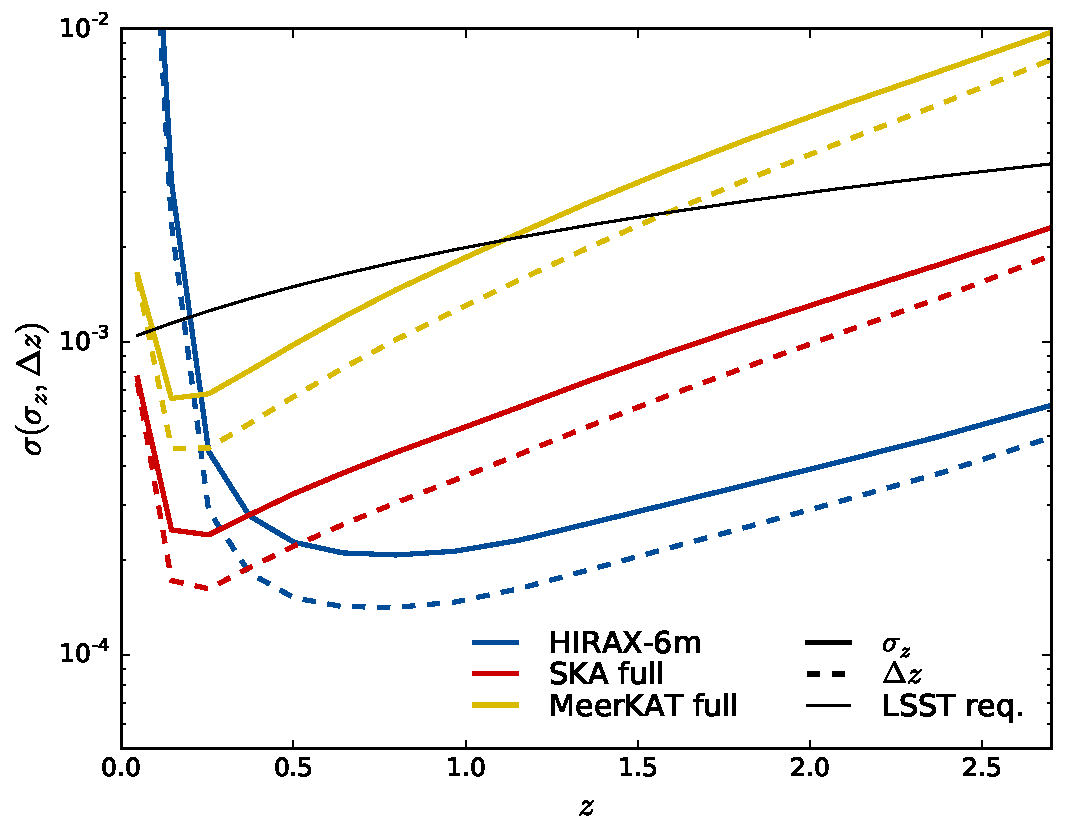
\includegraphics[width=0.49\textwidth]{compare_wbias}
      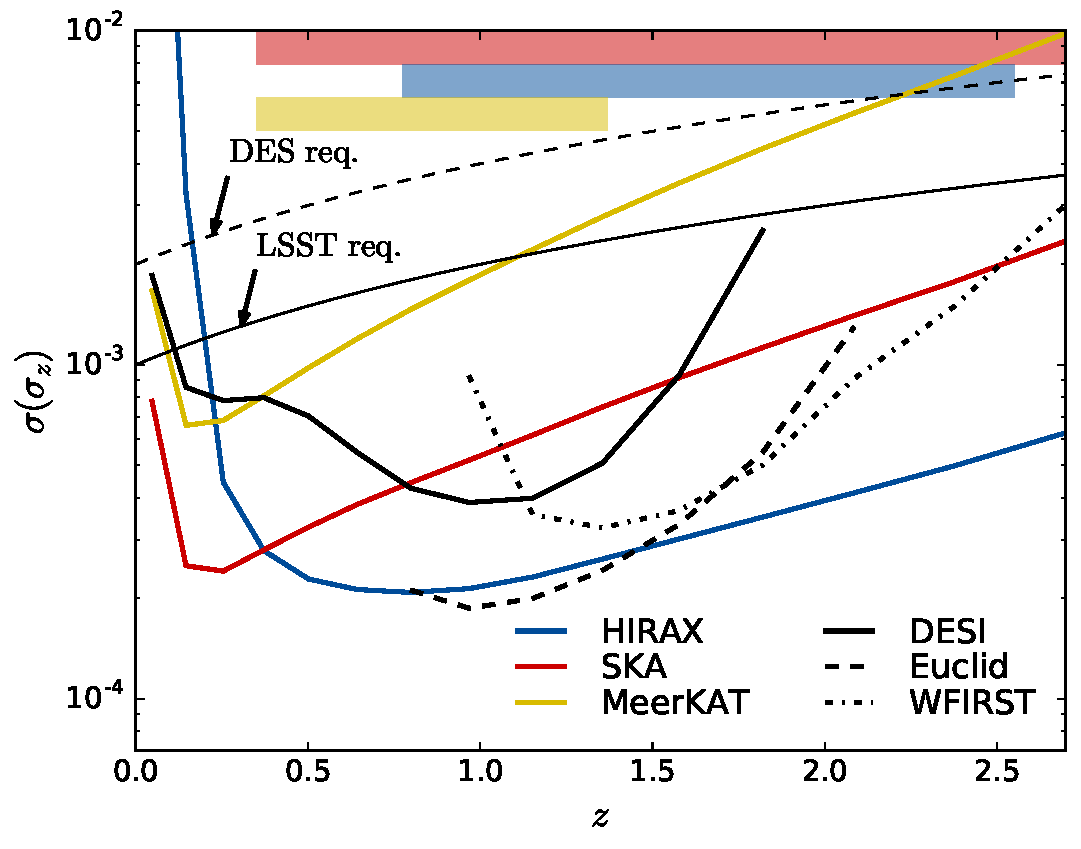
\includegraphics[width=0.49\textwidth]{compare_spec}
      \caption{\TODO{}}
      \label{fig:compare_spec}
    \end{figure*}
    Using the formalism described above, and in the simplified scenario of Gaussian photo-$z$s,
    we present, in the left panel of Figure \ref{fig:compare_spec}, the forecast constraints on the 
    photo-$z$ bias ($\Delta z$) and variance ($\sigma_z$) for the key intensity mapping experiments
    introduced in Section \ref{ssec:method.imap}. Two key features must be noted in this figure.
    First, the uncertainties grow steeply at low redshifts. This is due to the reduced number of
    modes available in that regime, associated with the smaller comoving volume and the impact of
    non-linearities on lower values of $k$. Secondly, the ratio between $\sigma(\sigma_z)$ and
    $\sigma(\Delta z)$ stays roughly constant ($\sim1.4$). This is compatible with the expected ratio
    between the uncertainties associated to the maximum-likelihood estimates of the mean and standard
    deviation of a Gaussian distribution from a finite number of samples
    ($\sigma(\sigma)/\sigma(\mu)=\sqrt{2}$). This result holds for most of the cases explored here
    (see Section \ref{ssec:results.foregrounds} for an exception), and thus we have omitted the
    curves for $\sigma(\Delta z)$ in most of the subsequent figures.
    
    The right panel of Fig. \ref{fig:compare_spec} compares the constraints achievable by IM
    experiments with those forecast for the spectroscopic surveys described in Section
    \ref{ssec:method.spec}.
    
    
    
    \begin{figure}
      \centering
      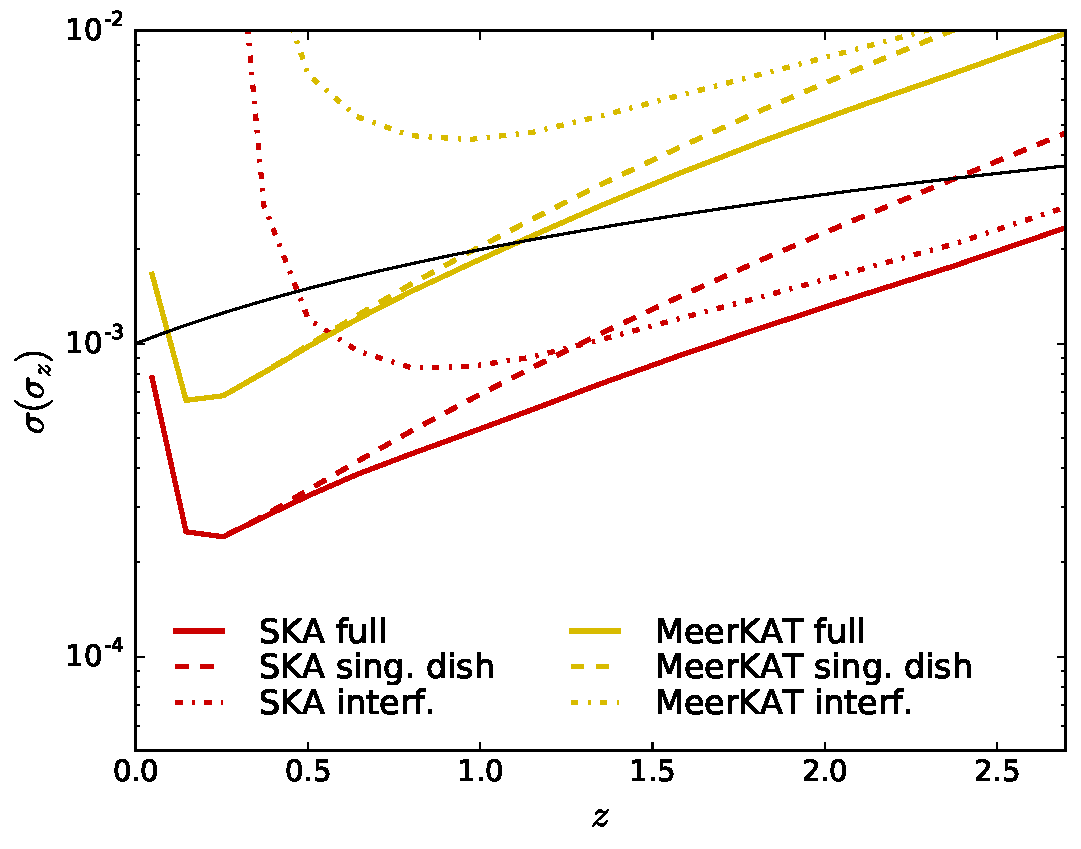
\includegraphics[width=0.49\textwidth]{compare_if_sd}
      \caption{\TODO{}}
      \label{fig:compare_if_sd}
    \end{figure}
    \begin{figure}
      \centering
      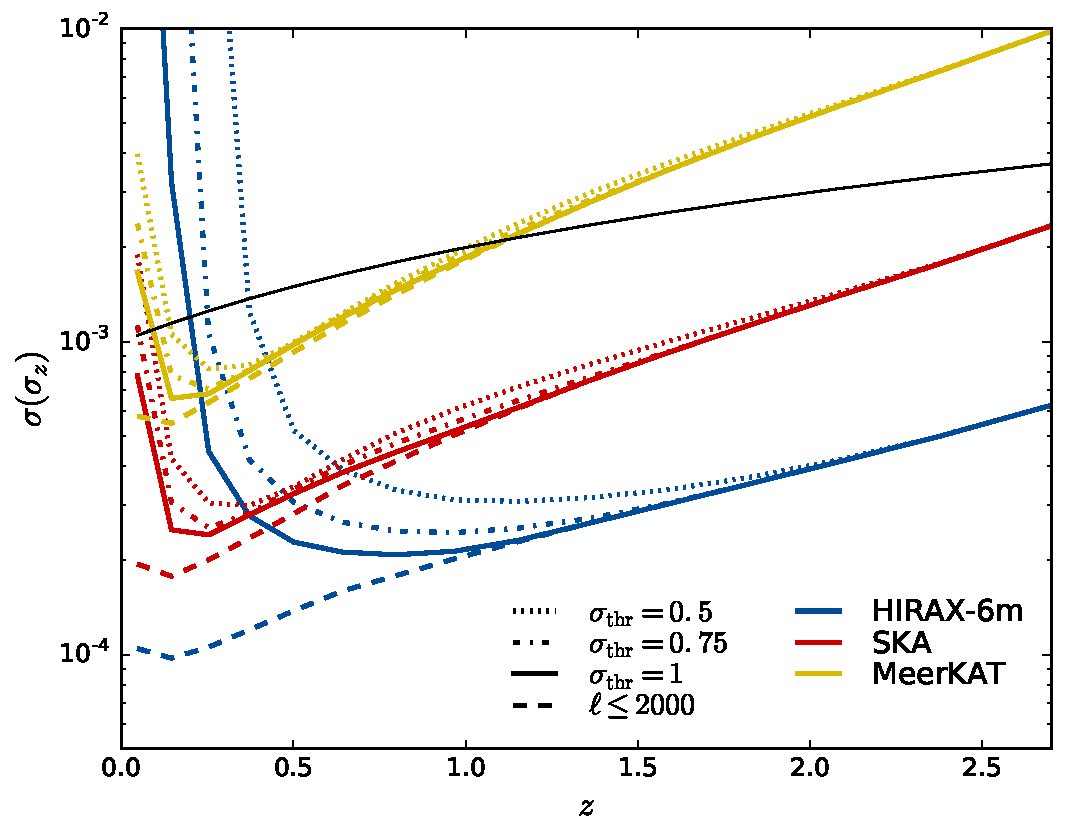
\includegraphics[width=0.49\textwidth]{compare_nlin}
      \caption{\TODO{}}
      \label{fig:compare_nlin}
    \end{figure}
    \begin{itemize}
     \item Comparison against spectroscopic surveys: left panel of Fig. \ref{fig:compare_spec}
     \item Constraints on $\sigma_z$ and $\Delta z$: right panel of Fig. \ref{fig:compare_spec}
     \item Interferometer vs single dish for SKA and MeerKAT: Fig. \ref{fig:compare_if_sd}
     \item Effect of non-linearities: Fig. \ref{fig:compare_nlin}
    \end{itemize}

    \TODO{
      \begin{itemize}
        \item Describe results for SKA and HIRAX in comparison with DESI, Euclid, WFIRST.
        \item Show forecasts on parameters before and after calibration.
      \end{itemize}
    }

  \subsection{Dependence on experimental parameters} \label{ssec:results.params}
    \TODO{
      \begin{itemize}
        \item Show results as a function of $f_{\rm sky}$, and noise level.
        \item Show results as a function of dish size for single-dish experiments
        \item Show results as a function of minimum baseline for interferometers
      \end{itemize}
    }

  \subsection{Foregrounds} \label{ssec:results.foregrounds}
    \TODO{
      \begin{itemize}
        \item Show results in the presence of foreground residuals.
        \item As a function of residual amplitude?
        \item Discuss correlated extragalactic foregrounds?
      \end{itemize}
    }

  \subsection{Generalized redshift distributions} \label{ssec:results.outliers}
    \TODO{
      \begin{itemize}
        \item Include hard-tail parameters (e.g. Cauchy contribution - Voigt profile).
        \item Non-parametric calibration. Show results for bins of $dN/dz$ of fixed
          width as a function of experiment and redshift.
      \end{itemize}
    }
    
  \subsection{Impact on cosmological constraints} \label{ssec:results.cosmo}
    \TODO{Show effect of achieved photo-$z$ priors on final cosmological parameters}

\section{Discussion}\label{ssec:discuss}
  \TODO{\lipsum[12]}

\section*{Acknowledgments}
  We thank Odin the almighty for useful comments and discussions.
 
\bibliography{paper}

\appendix
\begin{widetext}
  \section{Individual clustering redshifts}\label{app:ind_phz}
    \TODO{
      Possibly describe formalism to sharpen redshifts for individual redshifts.
    }
    
  \section{Angular power spectra}\label{app:cls}
    This section describes the theoretical models used for the angular power spectra entering
    the computation of the Fisher matrix (Eq. \ref{eq:fisher}).
    
    The cross-power spectrum between two tracers of the cosmic density field, $a$ and $b$,
    can be estimated as:
    \begin{equation}\label{eq:int_cl}
      C^{ab}_\ell=4\pi\int_0^\infty\frac{dk}{k}{\cal P}_\Phi(k)W^a_\ell(k)W^b_\ell(k),
    \end{equation}
    where ${\cal P}_\Phi(k)$ is the power spectrum of the primordial curvature perturbations
    and $W^a_\ell(k)$ is the window function for tracer $a$, containing information
    about the different contributions to the total anisotropy in that tracer and about
    its redshift distribution.
    
    In the case of galaxy clustering and intensity mapping, and neglecting contributions
    from magnification bias and large-scale relativistic effects, $W^a$ is given by:
    \begin{equation}
      W^a_\ell(k)=\int_0^\infty dz\,\phi_a(z)\left[b_a(z)T_\delta(k,z)j_\ell(k\chi(z))+
                   \frac{1+z}{H(z)}T_\theta(k,z)j''_\ell(k\chi(z))\right],
    \end{equation}
    where $H(z)$ and $\chi(z)$ are the expansion rate and radial comoving distance at
    redshift $z$ respectively, $\phi_a(z)$ is the source redshift distribution, and
    $T_\delta$ and $T_\theta$ are the transfer functions of the matter overdensity
    and velocity divergence fields. Note that, even though we include the effect of
    non-linearities using the non-linear transfer function for $\delta$ (through
    the prescription of \TODO{cite halofit}), we only introduce the effect of
    redshift-space distortions at the linear level, and only consider a deterministic
    linear bias $b_a(z)$. This is, nevertheless, a more rigorous treatment than has
    been used in the literature, and the procedure used to mitigate the effect of
    non-linearities described in Section \ref{ssec:method.fisher} should minimize
    the corresponding impact on the forecasts presented here.
    
    For galaxy shear tracers of weak lensing, the expression for the window function
    is:
    \begin{equation}
      W^a_\ell(k)=-\frac{1}{2}\sqrt{\frac{(\ell+2)!}{(\ell-2)!}}\int_0^\infty
      \frac{dz}{H(z)}\int_z^\infty dz'\phi_a(z')\frac{\chi(z')-\chi(z)}{\chi(z')\chi(z)}
      T_{\phi+\psi}(k,z)\,j_\ell(k\chi(z)),
    \end{equation}
    where $T_{\phi+\psi}$ is the transfer function for the sum of the two metric
    potentials in the Newtonian gauge.
    
    The computation of Eq. \ref{eq:int_cl} was carried out using a modified version of
    the Boltzmann code CLASS \TODO{cite}.
    
  \section{Noise power spectrum for intensity mapping experiments}\label{app:noise_im}
    \begin{figure}
      \centering
      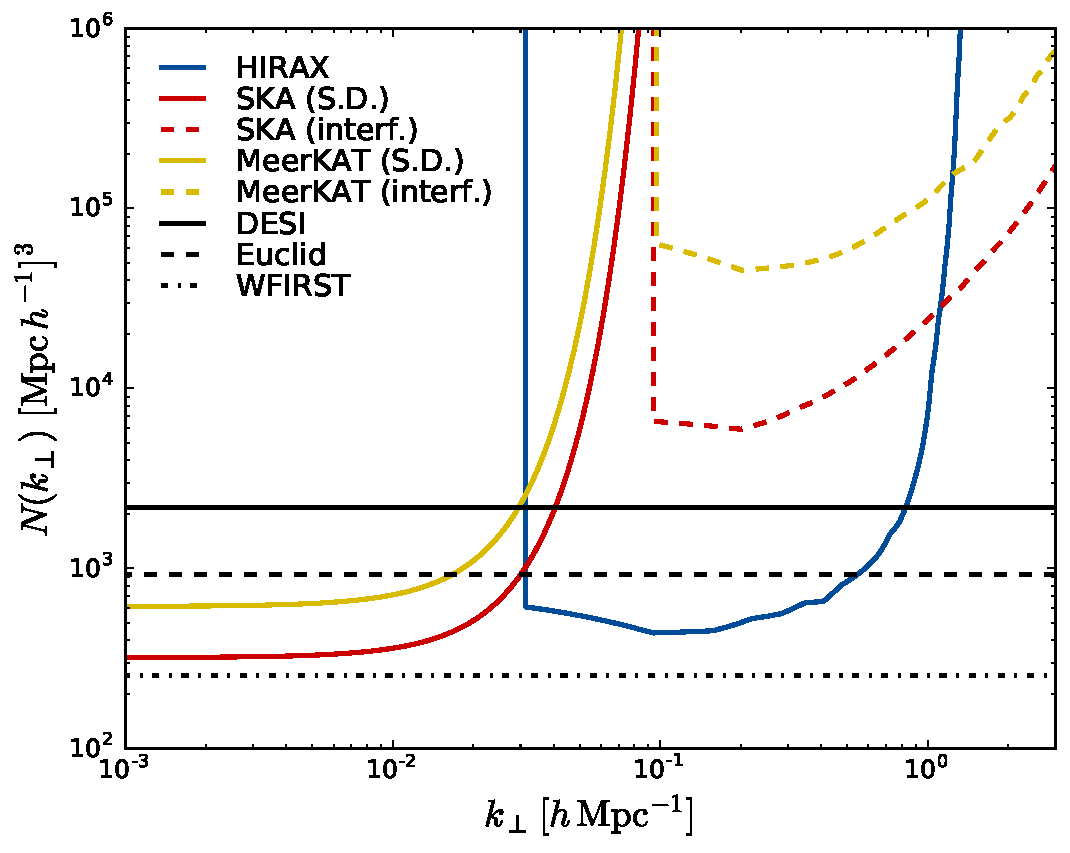
\includegraphics[width=0.49\textwidth]{nk}
      \caption{\TODO{}}
      \label{fig:nk}
    \end{figure}
    This section derives the expression for the noise power spectra of single-dish
    experiments and interferometers presented in Eq. \ref{eq:nl_im}
    \TODO{
      Power spectrum models used here
    }
  
  \section{Voigt profile}\label{app:voigt}
    A Voigt profile is given by a convolution of a Gaussian and a Cauchy or Lorentzian
    distribution, and is thus parametrized by the half-width at half-maximum of
    both component ($\gamma_G$ and $\gamma_L$ respectively here):
    \begin{align}\label{eq:voigt}
      p_V(x;\gamma_G,\gamma_L)\equiv&\int_{-\infty}^{\infty}dx' p_G(x';\gamma_G)\,p_L(x-x';\gamma_L),\\
      p_G(x;\gamma_G)\equiv\sqrt{\frac{{\rm ln} 2}{\pi\gamma_G^2}}\exp&\left[-{\rm ln}(2)x^2/\gamma_G^2\right],\hspace{12pt}
      p_L(x;\gamma_L)\equiv\frac{\gamma_L}{\pi}\frac{1}{\gamma_L^2+x^2}.
    \end{align}
    In order to avoid the computational complexity of evaluating Eq. \ref{eq:voigt}, we
    will use an approximate pseudo-Voigt profile:
    \begin{align}\label{eq:pvoigt}
      \tilde{p}_V(x;\gamma_G,\gamma_L)=\eta p_L(x;\bar{\gamma})+(1-\eta)\,p_G(x;\bar{\gamma}),
    \end{align}
    with expressions for $\eta$ and $\bar{\gamma}$ in terms of $\gamma_G$ and $\gamma_L$ given
    by \cite{pvoigt}:
    \begin{align}
      &\bar{\gamma}(\gamma_G,\gamma_L)=\left[\gamma_G^5+2.69269\gamma_G^4\gamma_L+2.42843\gamma_G^3\gamma_L^2 + 4.47163\gamma_G^2\gamma_L^3 + 0.07842\gamma_G\gamma_L^4 + \gamma_L^5\right]^{1/5},\\
      &\eta(\gamma_G,\gamma_L)=1.36603\frac{\gamma_L}{\bar{\gamma}}-0.47719\left(\frac{\gamma_L}{\bar{\gamma}}\right)^2+0.11116\left(\frac{\gamma_L}{\bar{\gamma}}\right)^3
    \end{align}

    The cumulative distribution entering the redshift distribution is:
    \begin{align}\nonumber
      \int_{z_b^i}^{z_b^f}dz_{\rm ph}p(z_{\rm ph}|z,\sigma_z,\gamma_L)=
      &\frac{\eta}{\pi}\left[{\rm arctan}\left(\frac{z_b^f-z}{\bar{\gamma}}\right)-{\rm arctan}\left(\frac{z_b^i-z}{\bar{\gamma}}\right)\right]\\
      &\frac{1-\eta}{2}\left[{\rm erf}\left(\frac{(z_b^f-z)\sqrt{{\rm ln}2}}{\bar{\gamma}}\right)-{\rm erf}\left(\frac{(z_b^i-z)\sqrt{{\rm ln}2}}{\bar{\gamma}}\right)\right]
    \end{align}


\end{widetext}

\end{document}
